\section{Optimization Methods}
One of the biggest challenges to maintain the stability of DAG system is that, 
as the local data structure growing, the graph algorithms ($Pivot()$, $MCMC()$, $StreamNetOrder()$), 
relies on some of the graph properties that needs to be recalculated everytime these functions are called,
which are very expensive. 
Table~\ref{tab:properties} list all the expensive graph properties that are called. 
Suppose the set of blocks in the DAG is represented by $B$, and the depth of the pivot chain is $d$.
Then we give the analysis of complexity in the following way. 
$Score()$ relies on the calculation of $SubTree()$ which is dependent on the breath first search ($BFS$), and the average $BFS$
complexity would be $O(|B|)$, consider the scenario of MCMC() and Pivot() which are advanced through the main chain,
the complexity would be in total $O(|B|*d)$ in both of these two cases.
The calculation of $Past()$ also relies on the $BFS$ operator, in the StreamNetOrder() algorithm, the complexity would be 
accrued to $O(|B| * d)$.
TopOrder() is used in sub-order ranking the blocks in the same epoch.
It's the classical topological sorting problem, and the complexity in the StreamNetOrder() would be $O(|B|)$.

\begin{table}[]
\caption {Analysis of Graph properties calculation} \label{tab:properties}
\begin{center}
\begin{tabular}{|l|l|l|l|}
\hline
Graph Property        & Algorithm used   & Complexity & Tot \\ \hline
Score(G, b)           & MCMC()           & $O(|B|)$              & $O(|B|*d)$  \\ \hline
Score(G, b)           & Pivot()          & $O(|B|)$              & $O(|B|*d)$  \\ \hline
Past(G,b) - Past(G,p) & StreamNetOrder() & $O(|B|)$          & $O(|B|*d)$  \\ \hline
TopOrder(G, b)        & StreamNetOrder() & $O(|B|)$              & $O(|B|)$    \\ \hline
\end{tabular}
\end{center}
\end{table}



Considering new blocks are genereted and merged into the local data structure in a streaming way.
The expensive graph properties could be maintained dynamically as the DAG grows.
Such that the complexity of calculating these properties would be armortized to each time a new block is generated or merged.
In the following sections, we will discuss how to design streaming algorithms to achieve this goal.

\subsection{Optimization of Score()}
In the optimized version, the DAG will have a map that keeps the score of each block. once there is a new generated/merged block,
it will trigger the BFS based UpdateScore() algorithm to update the scores of the block in the map that are referenced by the new block.
The skeleton of the UpdateScore() algorithm is as Algorithm~\ref{algo:update_score} shows.

\IncMargin{1em}
\begin{algorithm}
\SetKwData{Left}{left}\SetKwData{This}{this}\SetKwData{Up}{up}
\SetKwFunction{Union}{Union}\SetKwFunction{FindCompress}{FindCompress}
\SetKwInOut{Input}{input}\SetKwInOut{Output}{output}

\KwIn{ Graph $G$, Block $b$, Score map $S$}
\KwOut{ Updated score map $S$ }

    $Q = [b]$ \;
    $visited = \{\}$ \;
    \While{ $Q != \O$} {
        $b'$ = $Q.pop()$ \;
        \For { $b'' \in Before(G, b')$ } {
            \uIf{$b'' \notin visited \land b'' != \perp$} {
                $Q.append(b'')$ \;
                $visited.add(b'')$ \;
            }
        }
        $S[b'] ++$ \;
    }

\Return{$S$} \;

\caption{{\sc UpdateScore($G$, $b$).}}
\label{algo:update_score}
\end{algorithm}
\DecMargin{1em}


\subsection{Optimization of Past(G,b) - Past(G,p)}

We abbreviate the Past(G,b) - Past(G,p) as GetDiffSet(G,b,C) which is shown in the Algorithm~\ref{algo:get_diff_set}.
This algorithm is in essence a dual direction $BFS$ algorithm. Starting from the block $b$, it will traverse its referenced blocks.
Every time a new reference block $b'$ is discovered, it will perform a backward $BFS$ to `look back' to see if itself is already covered by the $b$'s parent block of $p$. 
If yes, $b'$ would not be added to the forward $BFS$ queue.  
To avoid the complexity of the backward $BFS$, the previous calculated diff set will be added to the covered set $C$, which will be passed to GetDiffSet() as a parameter.
To be more specific, when a backward BFS is performed, the blocks in $C$ will not be added to the search queue.
This backward search algorihtm is denoted as IsCovered() and described in detail in Algorithm~\ref{algo:is_covered}.

Figure~\ref{get_diff} shows the example of the GetDiffSet() method for block $5$.
it first perform forward BFS to find block $4$ which does not have children, then it will be added to the diff set.
$4$ then move forward to $1$, which have three childrens, if it detect $3$ which is the parent of $5$, it will stop searching prompty.
If it continue searching on $2$ or $4$, these two blocks would not be added to the search queue, because they are already in the covered set.

\IncMargin{1em}
\begin{algorithm}
\SetKwData{Left}{left}\SetKwData{This}{this}\SetKwData{Up}{up}
\SetKwFunction{Union}{Union}\SetKwFunction{FindCompress}{FindCompress}
\SetKwInOut{Input}{input}\SetKwInOut{Output}{output}

\KwIn{ Graph $G$, Block $b$, covered block set $C$}
\KwOut{ diff set $D \gets Past(G,b) - Past(G,p)$ }

    $D = {\O}$ \;
    $Q \gets [b]$ \;
    $visited = \{b\}$ \;
    $p$ = $Parent(G, b)$ \;
    \While{ $Q != \O$} {
        $b'$ = $Q.pop()$ \;
        \For { $b'' \in Before(G, b')$ } {
            \uIf{$IsCovered(G, p ,b'',C) \land b'' != \perp$} {
                $Q.append(b'')$ \;
                $visited.add(b'')$ \;
            }
        }
        $D.add(b')$ \;
        $C.add(b')$ \;
    }

\Return{$D$} \;

\caption{{\sc GetDiffSet($G$, $b$, $C$).}}
\label{algo:get_diff_set}
\end{algorithm}
\DecMargin{1em}


\IncMargin{1em}
\begin{algorithm}
\SetKwData{Left}{left}\SetKwData{This}{this}\SetKwData{Up}{up}
\SetKwFunction{Union}{Union}\SetKwFunction{FindCompress}{FindCompress}
\SetKwInOut{Input}{input}\SetKwInOut{Output}{output}

\KwIn{ Graph $G$, Block $b'$, parent $p$, covered block set $C$}
\KwOut{true if covered by parent, else false }
    $Q \gets [b']$ \;
    $visited = \{b\}$ \;
    \While{ $Q != \O$} {
        $b''$ = $Q.pop()$ \;
        \For { $ t \in Child(G, b'')$ } {
            \uIf{$t=p$}{
                return true \;
            }
            \uElseIf{$t \notin visited \land t \notin C$} {
                $Q.add(t)$ \;
                $visited.add(t)$ \;
            }
        }
    }

\Return{false} \;

\caption{{\sc IsCovered($G$, $p$, $b'$, $C$).}}
\label{algo:is_covered}
\end{algorithm}
\DecMargin{1em}


\begin{figure}[!ht]
\begin{center}
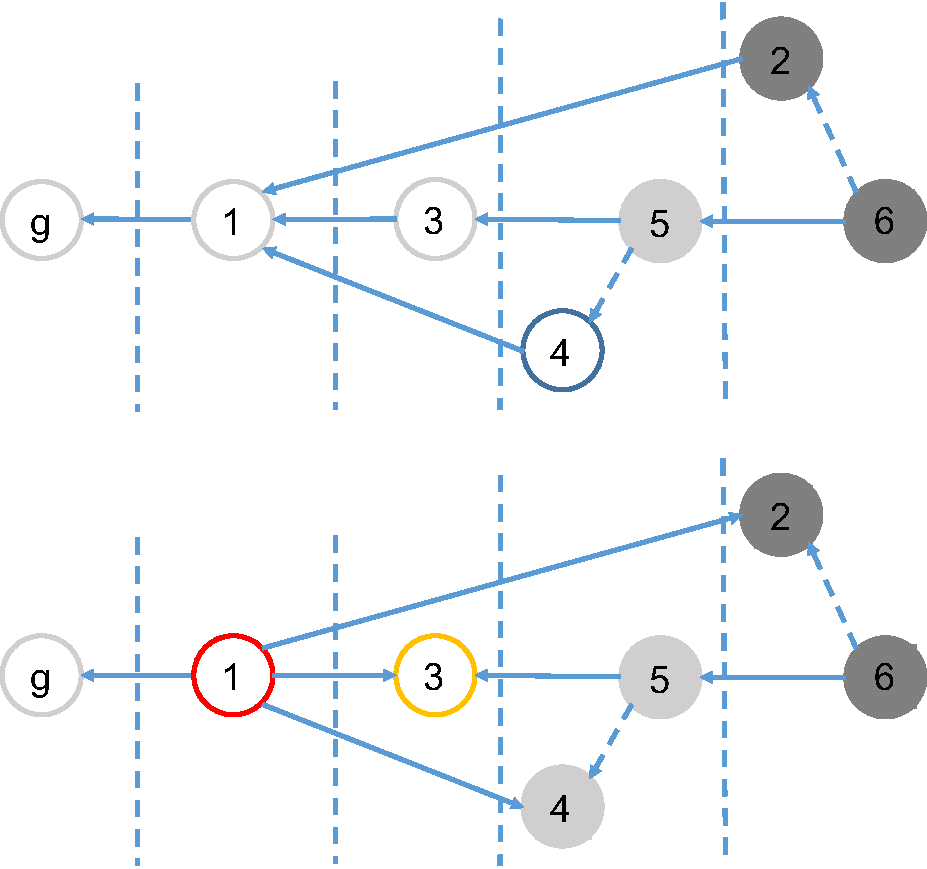
\includegraphics[width=0.35\textwidth]{figures/get_diff.pdf}
    \caption{
        Example of the streaming get diff set method.
     }
\label{get_diff}
\end{center}
\end{figure}

\subsection{Optimization of TopOrder()}
The topological order is used in sorting the blocks in the same epoch.
To get the toppological order, every time, there needs a top sort of the whole DAG from the scratch.
However we can easily update the topological order when a new block is added or merged.
 The update rule is, when a new block is added, it's topological position will be $TopScore(G, b) \gets min(TopScore(G, Parent(b)), TopScore(G, Reference(b)))$. This step can be done in $O(1)$ 


To summarize, the optimized streaming operators can achieve the performance improvement as Table~\ref{tab:improvement} shows. 

\begin{table}[]
\caption {Analysis of Graph properties calculation} \label{tab:improvement}
\begin{center}
\begin{tabular}{|l|l|l|l|}
\hline
Graph Property        & Algorithm used   & Complexity & Tot \\ \hline
Score(G, b)           & MCMC()           & $O(|B|)$              & $O(d)$  \\ \hline
Score(G, b)           & Pivot()          & $O(|B|)$              & $O(d)$  \\ \hline
Past(G,b) - Past(G,p) & StreamNetOrder() & $O(|B|)$          & $O(|B|)$  \\ \hline
TopOrder(G, b)        & StreamNetOrder() & $O(|1|)$              & $O(|1|)$    \\ \hline
\end{tabular}
\end{center}
\end{table}



%\subsection{Genesis Snapshot}
